\section{Optimization}
This problem was solved in group with Enrique Saiz.\\
The optimization problem was to find the best new places for recycling containers. The problem has to take in account the positions of actual recycling contains as well as geographic data of the city of Kaunas.\\
\subsection{Data used}
We get the data from \url{https://open-data-ls-osp-sdg.hub.arcgis.com/datasets/}, and then we extracted and filtered the data with geopandas python library, and we converted all the geographic coordinates that used EPSG:3346 to common EPSG:4326.
We chose to use the population data and relevants economic secotrs in our opinion (primary and secondary sectors, construction, commerce, food sector).\\
\begin{figure}[H]
    \centering
    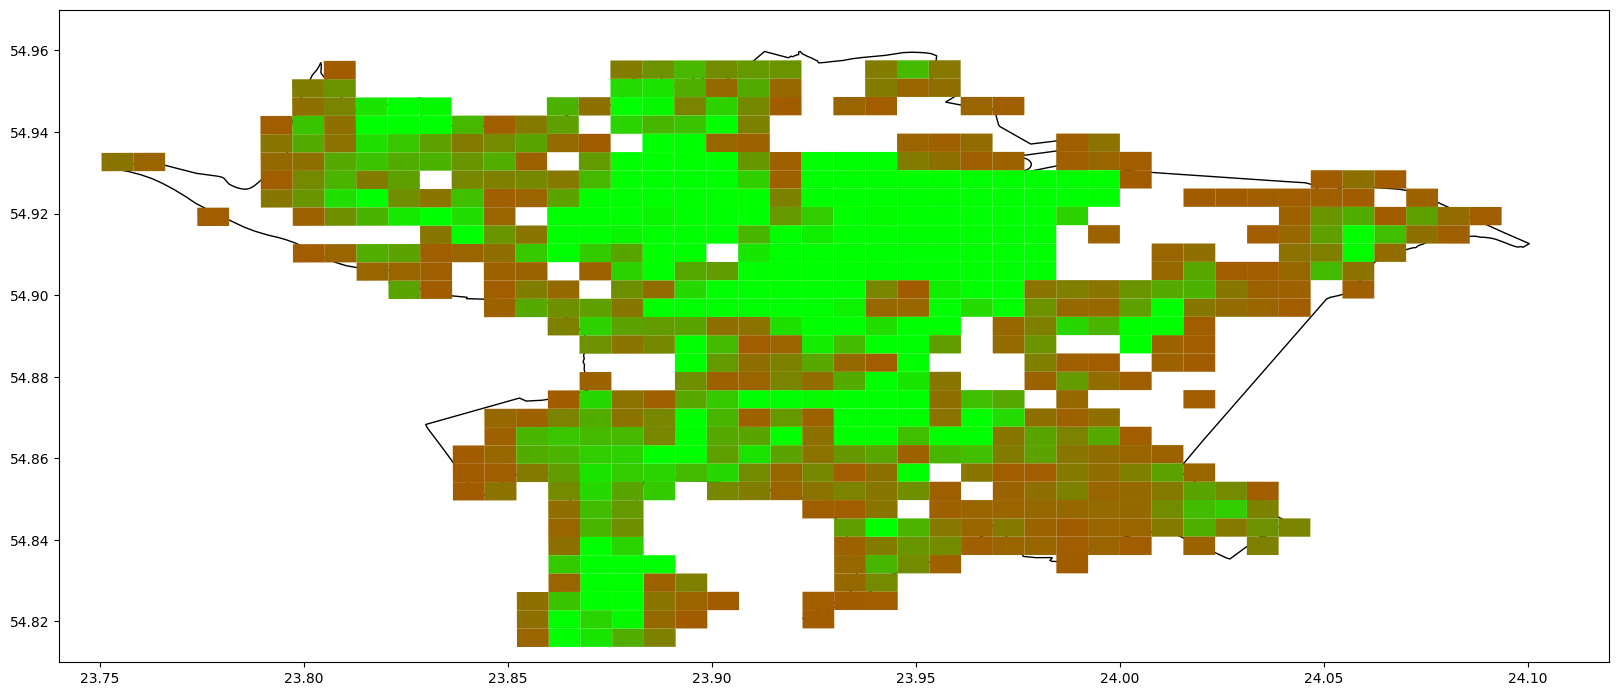
\includegraphics[width=8cm]{images/part3/newpopnormalised.png}
    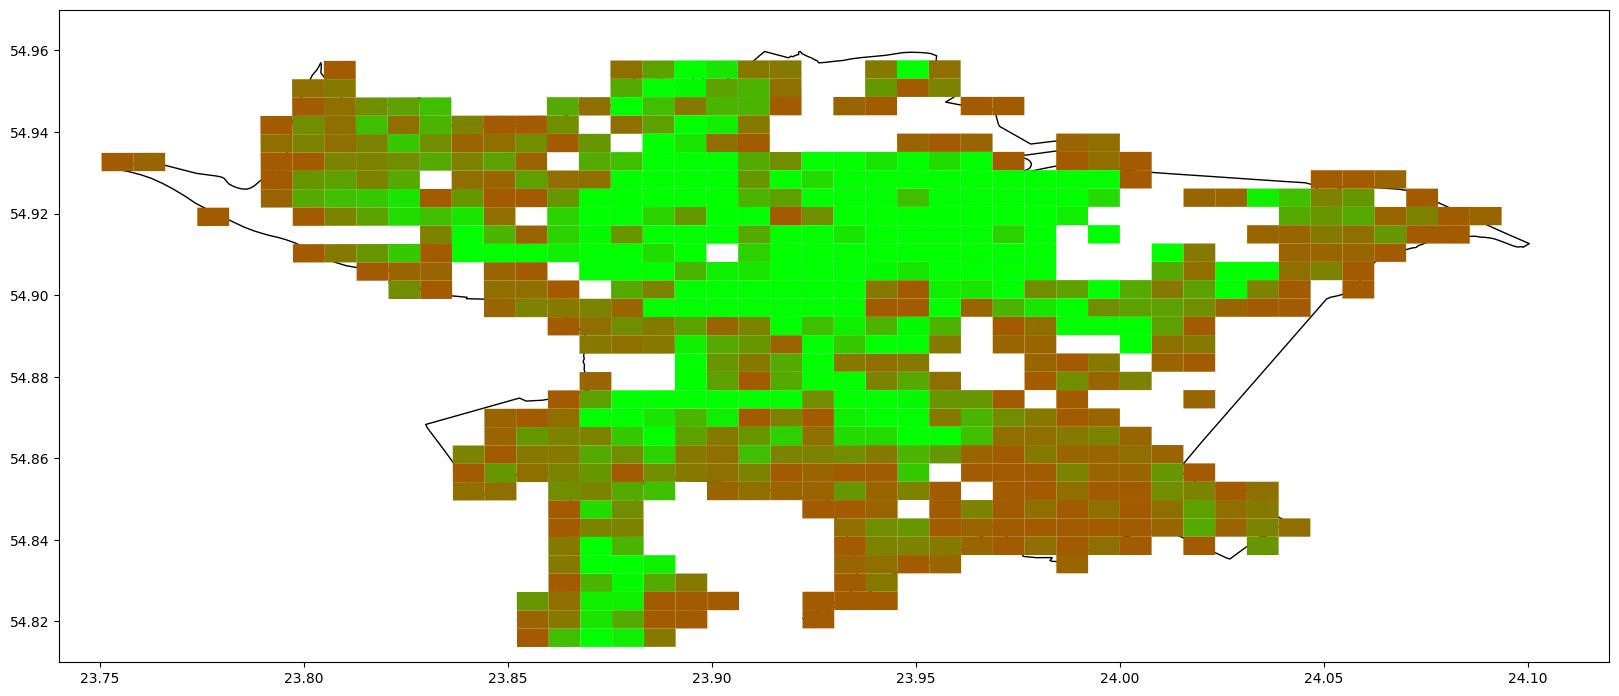
\includegraphics[width=8cm]{images/part3/neweconormalised.png}
    \caption{Plots of the population and the economic activity in Kaunas}
    \label{fig:economicandpop}
\end{figure}
And then, we normalised and merged the data to get a region of interest.\\
\begin{figure}[H]
    \centering
    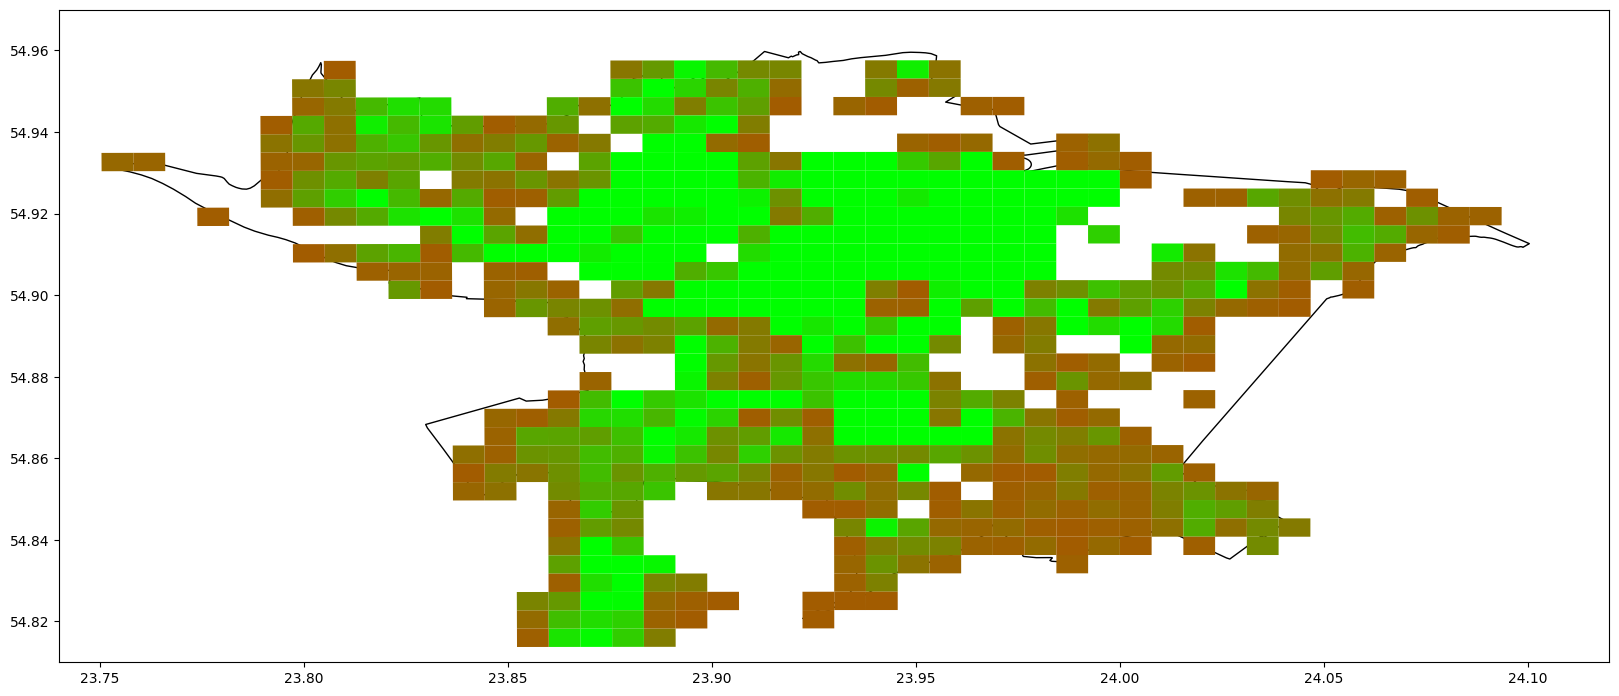
\includegraphics[width=10cm]{images/part3/newnormalised.png}
    \caption{Plot of the normalised region of interest}
    \label{fig:normaliseddata}
\end{figure}
\subsection{Creation of new containers}
So, at the beginning we had 567 recycling spots, and we want to add 10 more according to our data :\\
- Population and relevant sectors in each area\\
- Distance between points as uniform as possible\\
So first we spawn 10 random points in our region of interest (according to the positions of the existing containers).
\begin{lstlisting}[language=Python, style=jupycolors]
# generate and initialize random free positions, to be optimized with gradient descent
new = 10

x_values = np.random.uniform(min(positionsFixed[:, 0]), max(positionsFixed[:, 0]), new)
y_values = np.random.uniform(min(positionsFixed[:, 1]), max(positionsFixed[:, 1]), new)
positionsFree = np.column_stack((x_values, y_values))

originalPositionsFree = positionsFree.copy()

visualization(positionsFixed, positionsFree)
\end{lstlisting}
\begin{figure}[H]
    \centering
    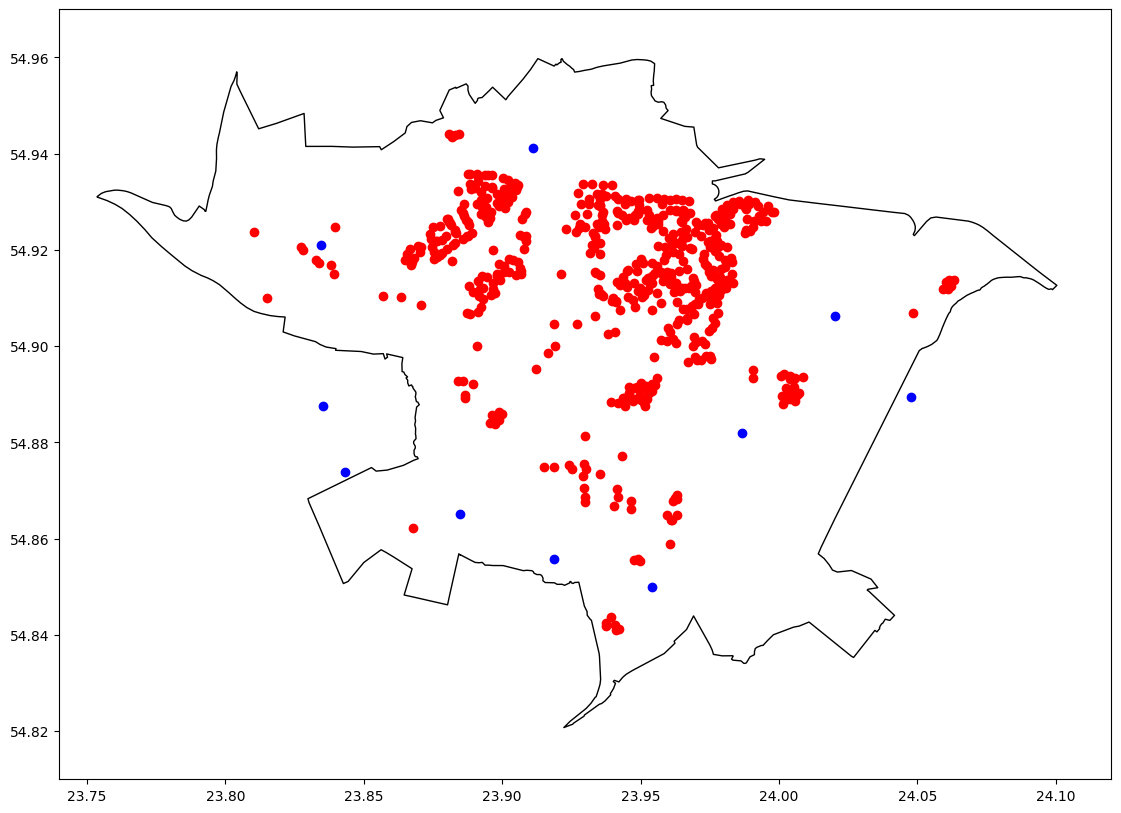
\includegraphics[width=10cm]{images/part3/pointsNewRandom.png}
    \caption{Creation of 10 new points (in blue)}
    \label{fig:newpoints}
\end{figure}
\subsection{Optimization of new containers}
So to opitmize the positions of the new conntainers, we created an objective function that has its minimum when all the points have the minimal distance between all and are more present in the region of interest.
We tried many combinations of the data (multiplications, use of some factors), comparing what had more weight (and what should have more), and we finally found this combination that worked well and give results that seems accurate.
\begin{lstlisting}[language=Python, style=jupycolors]
def objectiveFunctDistanceImportance(positionsFixed, positionsFree):
    distanceVal = 0
    importanceVal = 0
    avgDist = averageDistanceBetweenAllPoints(positionsFixed, positionsFree)
    
    # distance value
    for i in range(0, len(positionsFixed)):
        for j in range(0, len(positionsFree)):
            edgeDistance = distanceBetweenTwoPoints(positionsFixed[i], positionsFree[j])
            distanceVal += (avgDist - edgeDistance)**2

    for i in range(0, len(positionsFree)):
        for j in range(i+1, len(positionsFree)):
            edgeDistance =  distanceBetweenTwoPoints(positionsFree[i], positionsFree[j])
            distanceVal += (avgDist - edgeDistance)**2

    # point value
    for i in range(0, len(positionsFree)):
        importanceVal += 1-float(get_normalized_value_at_coordinates(geo_data_merged, positionsFree[i, 0], positionsFree[i, 1]))
    
    return distanceVal + importanceVal
\end{lstlisting}
To find the minimum of this function, we will need an approximation of the gradient. $h$ is small enough to be a gradient approximation, but big enough to depend on the geographic data (it is 500x500m areas).
\begin{lstlisting}[language=Python, style=jupycolors]
def quasiGradient(positionsGiven, positionsNew, objectiveFunction, h=0.01):
    f0 = objectiveFunction(positionsGiven, positionsNew)
    df = positionsNew * 0
    for i in range(0, len(positionsNew)):
        for j in range (0, 2): # x and y coordinates
            positionsFreeNew = positionsFree; 
            positionsFreeNew[i][j] += h
            f1 = objectiveFunction(positionsGiven, positionsFreeNew) #changed from positionsFixed
            df[i][j] = (f1-f0)/h
    return df
\end{lstlisting}
And finally, we use the gradient descend method to find the minimum of the objective function.
\begin{lstlisting}[language=Python, style=jupycolors]
def quasiGradientDescent(positionsFixed, positionsFree, objectiveFunction, step=0.02, eps=1e-3, maxIter=1000):
    iter = 0
    objValOld = objectiveFunction(positionsFixed, positionsFree)
    objValNew = objValOld
    print("initial: ", objValOld)
    grad = quasiGradient(positionsFixed, positionsFree, objectiveFunction)
    while np.linalg.norm(grad) > eps and iter < maxIter and step > eps:
        grad = grad/np.linalg.norm(grad)
        print("grad", step, grad)
        positionsFree -= step * grad
        objValNew = objectiveFunction(positionsFixed, positionsFree) 
        if objValOld < objValNew:
            positionsFree += step * grad
            step = step * 0.9
        else:
            objValOld = objValNew
        grad = quasiGradient(positionsFixed, positionsFree, objectiveFunction)
        iter += 1
    print("iterations: ", iter,"/",maxIter)
    print("after optimization: ", objValNew)

    objectiveFunction(positionsFixed, positionsFree)
    visualization(positionsFixed, positionsFree, originalPositionsFree, True)

\end{lstlisting}
To optimize the new points, we just call the function like this.
\begin{lstlisting}[language=Python, style=jupycolors]
positionsFree = originalPositionsFree.copy()
quasiGradientDescent(positionsFixed, positionsFree, objectiveFunctDistanceImportance, maxIter=30)
\end{lstlisting}
\begin{figure}[H]
    \centering
    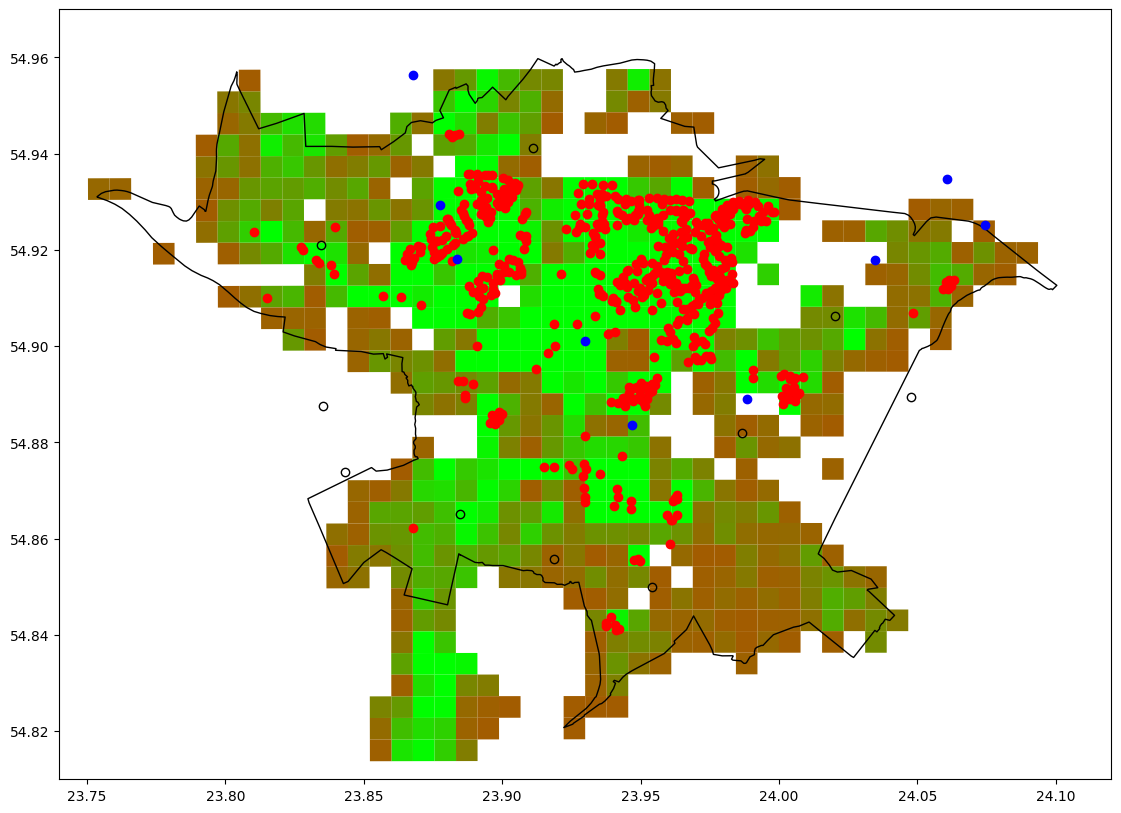
\includegraphics[width=8cm]{images/part3/pointsNewAfterGradient.png}
    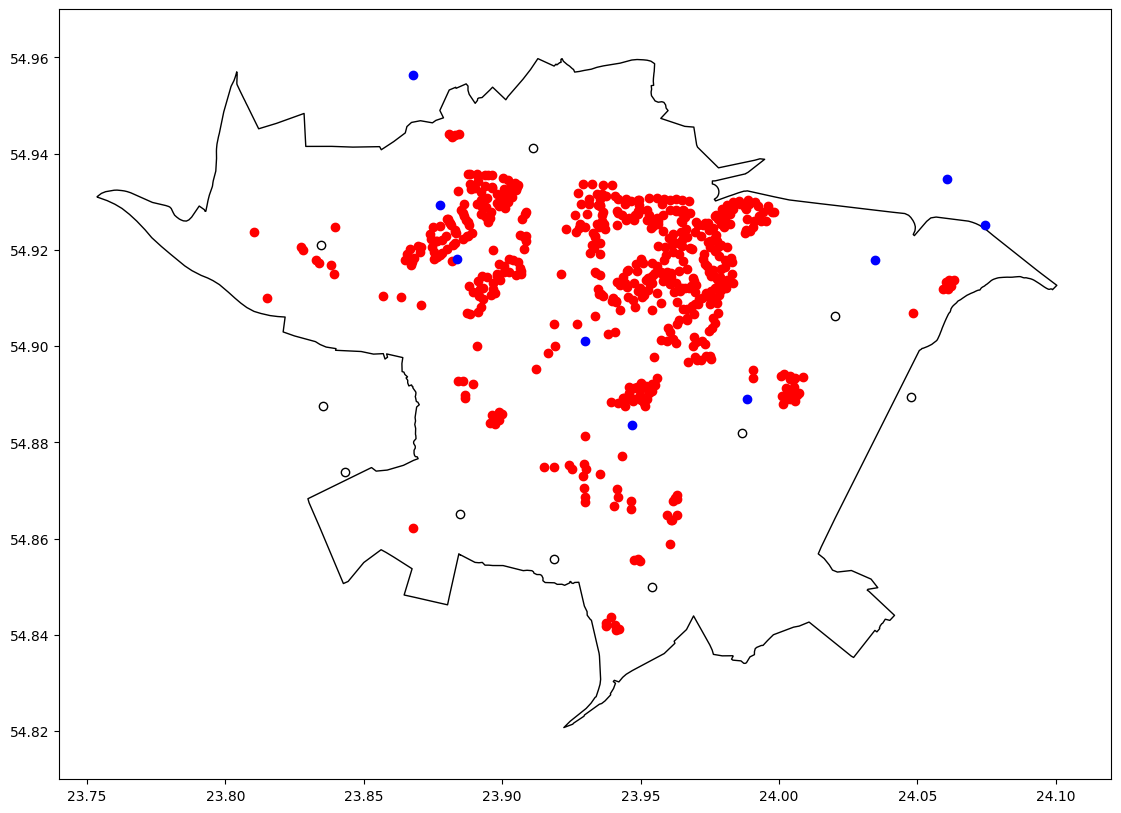
\includegraphics[width=8cm]{images/part3/pointsNewAfterGradwithoutecopop.png}
    \caption{Optimized new points (in blue), with their initial position (black circles)}
    \label{fig:newoptimized}
\end{figure}
By comparing the objective function at the points in their original positions and in their new positions, we see that the value decreased  as intended.
\begin{resultbox}
initial:  13.49093762170164\\
after optimization:  10.698442833207066
\end{resultbox}

\subsection{Future improvements}
Here is a small list of what we could improve on this algorithm in the future:\\
- Incorporate more features in objective function \\
- Differentiate the types of current recycling spots \\
- Repeat computations in high performance environment with 100x100 grid \\
- Visit and evaluate the new designated spots
